\documentclass[letterpaper]{article}
\usepackage{settings/aaai20}
\usepackage{times}
\usepackage{helvet}
\usepackage{courier}
\frenchspacing
\setlength{\pdfpagewidth}{8.5in}
\setlength{\pdfpageheight}{11in}

\usepackage{url}
\usepackage{graphicx}
\graphicspath{{./images}}
\usepackage{tabularx}
\usepackage{subfig}
\usepackage{multirow}
\usepackage{rotate}
\usepackage{array}
\renewcommand{\arraystretch}{1}
\newcolumntype{R}[1]{>{\raggedleft\arraybackslash}m{#1}}
\newcolumntype{C}[1]{>{\centering\arraybackslash}m{#1}}
\newcolumntype{L}[1]{>{\raggedright\arraybackslash}m{#1}}

%\usepackage{algorithm} 
\usepackage{algorithmic}
\usepackage[ruled,vlined,linesnumbered]{algorithm2e}
\makeatletter
\algocf@newcmdside@kobe{Procb}{%
	\KwSty{Procedure \normalfont\texttt{DL8.5-Recurse}$(I, init\_ub)$}%
	\ifArgumentEmpty{#1}\relax{ #1}
	\algocf@block{#2}{end}{#3}%
	\par
}

\algocf@newcmdside@kobe{Proca}{%
	\KwSty{Procedure \normalfont\texttt{DL8.5-Recurse}$(I)$}%
	\ifArgumentEmpty{#1}\relax{ #1}
	\algocf@block{#2}{end}{#3}%
	\par
}
\makeatother


\title{Learning Optimal Decision Trees Using Caching Branch-and-Bound Search}
\author{Gael Aglin, Siegfried Nijssen, Pierre Schaus\\
	\{firstname.lastname\}@uclouvain.be\\
	ICTEAM, UCLouvain\\
	Louvain-la-Neuve, Belgium}

\begin{document}
	\maketitle
	\begin{abstract}
	Several recent publications have studied the use of Mixed Integer Programming (MIP) for finding an optimal decision tree, that is, the best decision tree under formal requirements on accuracy, fairness or interpretability of the predictive model. These publications used MIP to deal with the hard computational challenge of finding such trees. In this paper, we introduce a new efficient algorithm, DL8.5, for finding optimal decision trees, based on the use of itemset mining techniques. We show that this new approach outperforms earlier approaches with several orders of magnitude, for both numerical and discrete data, and is generic as well. The key idea underlying this new approach is the use of a cache of itemsets in combination with branch-and-bound search; this new type of cache also stores results for parts of the search space that have been traversed partially.
\end{abstract}
	\section{Introduction}
Decision trees are among the most widely used machine learning models. Their success is due to the fact that they are simple to interpret and that there are efficient algorithms for learning trees of acceptable quality.

The most well-known algorithms for learning decision trees, such as CART \cite{breiman,quinlan:1993c4}, are greedy in nature: they grow the decision tree top-down, iteratively splitting the data into subsets.

While in general these algorithms learn models of good accuracy, their greedy nature, in combination with the NPhardness of the learning problem \cite{laurent:1976constructing}, implies that the trees that are found are not necessarily optimal. As a result, these algorithms do not ensure that:

\begin{itemize}
	\item the trees found are the most accurate for a given limit on
	the depth of the tree; as a result, the paths towards decisions may be longer and harder to interpret than necessary;
	\item  the trees found are the most accurate for a given lower
	bound on the number of training examples used to determine class labels in the leaves of the tree;
	\item the trees found are accurate while satisfying additional constraints such as on the fairness of the trees: in their predictions, the trees may favor one group of individuals over another.
\end{itemize}

With the increasing interest in explainable and fair models in machine learning, recent years have witnessed a renewed interest in alternative algorithms for learning decision trees that can provide such optimality guarantees.

Most attention has been given in recent years and in prominent venues to approaches based on mixed integer programming \cite{bertsimas:2017optimal,verwer:2019learning,aghaei:2019learning}. In these approaches, a limit is imposed on the depth of the trees that can be learned and a MIP solver is used to find the optimal tree under well-defined constraints.

However, earlier algorithms for finding optimal decision trees under constraints have been studied in the literature, of which we consider the DL8 algorithm of particular interest \cite{nijssen:2007mining,nijssen:2010optimal}. The existence of this earlier work does not appear to have been known to the authors of the more recent MIP-based approaches, and hence, no comparison with this earlier work was carried out.

DL8 is based on a different set of ideas than the MIP-based approaches: it treats the paths of a decision tree as itemsets, and uses ideas from the itemset mining literature \cite{agrawal:1996quest} to search through the space of possible paths efficiently, performing dynamic programming over the itemsets to construct an optimal decision tree. Compared to the MIP-based approaches, which most prominently rely on a constraint on depth, DL8 stresses the use of a minimum support constraint to limit the size of the search space. It was shown to support a number of different optimization criteria and constraints that do not necessarily have to be linear.

In this paper, we present a number of contributions. We will demonstrate that DL8 can also be applied in settings in which MIP-based approaches have been used; we will show that, despite its age, it outperforms the more modern MIP-based approaches significantly, and is hence an interesting starting point for future algorithms.

Subsequently, we will present DL8.5, an improved version of DL8 that outperforms DL8 by orders of magnitude. Compared to DL8, DL8.5 adds a number of novel ideas:

\begin{itemize}
	\item it uses branch-and-bound search to cut large additional parts of the search space;
	\item it uses a novel caching approach, in which we store also store information for itemsets for which the search space has been cut; this allows us to avoid redundant computation later on as well;
	\item we consider a range of different branching heuristics to find good trees more rapidly;
	\item the algorithm has been made any-time, i.e. it can be stopped at any time to report the best tree it has found so far.
\end{itemize}

In our experiments we focus our attention on traditional decision tree learning problems with little other constraints, as we consider these learning problems to be the hardest. How ever, we will show that DL8.5 remains sufficiently close to DL8 that the addition of other constraints or optimization criteria is straightforward.

In a recent MIP-based study, significant attention was given to the distinction between binary and numerical data \cite{verwer:2019learning}. We will show that DL8.5 outperforms this method on both types of data.

Our implementation is publicly available at \url{https://github.com/aglingael/dl8.5} and can easily be used from Python.

This paper is organized as follows. The next section presents the state of the art of optimal decision trees induction. Then we present the background on which our work relies, before presenting our approach and our results.
	\section{Related work}
In our discussion of related work, we will focus our attention on alternative methods for finding optimal decision trees, that is, decision trees that achieve the best possible score under a given set of constraints.

%\citeauthoryear{gf}{1336}
Most attention has been given in recent years to MIP-based approaches. \cite{bertsimas:2017optimal} %Bertsimas and Dunn (2017) 
developed an approach for finding decision trees of a maximum depth K that optimize misclassification error. They use K to model the problem in a MIP model with a fixed number of variables; a MIP solver is then used to find the optimal tree.

\cite{verwer:2019learning} %Verwer and Zhang (2019)
proposed BinOCT, an optimization of this approach, focused on how to deal with numerical data. To deal with numerical data, decision trees need to identify thresholds that are used to separate examples from each other. A MIP model was proposed in which fewer variables are needed to find high-quality thresholds; consequently, it was shown to work better on numerical data.

A benefit of MIP-based approaches is that it is relatively easy from a modeling perspective to add linear constraints or additional linear optimization criteria. \cite{aghaei:2019learning} %Aghaei, Azizi, and Vayanos (2019)
exploit this to formalize a learning problem that also takes into account the fairness of a prediction.

\cite{verwer:2019learning} %Verhaeghe et al. (2019)
recently proposed a Constraint Programming (CP) approach to solve the same problem. It supports a maximum depth constraint and a minimum support constraint, but only works for binary classification tasks. It also relies on branch-and-bound search and caching, but uses a less efficient caching strategy. The approach in the present paper is easily implemented and understood without relying on CP systems.

Another class of methods for learning optimal decision trees is that based on SAT Solvers \cite{narodytska:2018verifying,bessiere:2009minimising}. SAT-based studies, however, focus on a different type of decision tree learning problem than the MIP-based approaches: finding a decision tree of limited size that performs 100\% accurate predictions on training data. These approaches solve this problem by creating a formula in conjunctive normal form, for which a satisfying assignment would represent a 100\% accurate decision tree. We believe there is a need for algorithms that minimize the error, and hence we focus on this setting.

Most related to this work is the work of \cite{nijssen:2007mining,nijssen:2010optimal} %Nijssen and Fromont (2007; 2010)
on DL8, which relies on a link between learning decision trees and itemset mining. Similarly to MIP-based approaches, DL8 allows to find optimal decision trees minimizing misclassification error. DL8 does not require a depth constraint; it does however assume the presence of a minimum support constraint, that is, a constraint on the minimum number of examples falling in each leaf. In the next section we will discuss this approach in more detail. This discussion will show that DL8 can easily be used in settings identical to those in which MIP and CP solvers have been used. Subsequently, we will propose a number of significant improvements, allowing the itemset-based approach to outperform MIP-based and CP-based approaches.


	\section{Background}
\subsection{Itemset mining for decision trees}
We limit our discussion to the key ideas behind DL8, and assume that the reader is already familiar with the general concepts behind learning decision trees.

DL8 operates on Boolean data. As running example of such data, we will use the dataset of Table 1a, which consists of three Boolean features and eleven examples. The optimal decision tree for this database can be found in Figure 1a. While it may seem a limitation that DL8 only operates on Boolean data, there are straightforward ways to transform any tabular database in a Boolean database: for categorical attributes, we can create a Boolean column for each possible value of that attribute; for numerical attributes, we can create Boolean columns for possible thresholds for that attribute.

DL8 takes an itemset mining perspective on learning decision trees. In this perspective, the binary matrix of Table 1a is transformed into the transactional database of Table \ref{tab:1b}. Each transaction of the dataset contains an itemset describing the presence or absence of each feature in the dataset. More formally, the database $\mathcal{D}$ can be thought of as a collection $\mathcal{D} = \{(t, I, c)\;|t\in \mathcal{T} , I \subseteq \mathcal{I}, c \in \mathcal{C}\}$, where $\mathcal{T}$ represents the transaction or rows identifiers, $\mathcal{I}$ is the set of possible items, and $\mathcal{T}$ is the set of class labels; within $\mathcal{I}$ there are two items (one positive, the other negative) for each original Boolean feature, and each itemset $I$ contains either a positive or a negative item for every feature.

\begin{table}
	\subfloat[subcaption]{
		\begin{tabular}{c|c|c||c}
			\hline
			A		&	B	&	C	&	classe		\\
			\hline
			0		&	1	&	1	&	0			\\
			1		&	0	&	1	&	1			\\
			0		&	0	&	1	&	1			\\
			0		&	1	&	0	&	0			\\
			1		&	0	&	0	&	1			\\
			0		&	0	&	0	&	0			\\
			0		&	0	&	1	&	0			\\
			1		&	1	&	0	&	1			\\
			0		&	0	&	0	&	1			\\
			0		&	0	&	1	&	0			\\
			0		&	0	&	0	&	1			\\
			\hline
		\end{tabular}
	}~
	\subfloat[Transactional database]{
		\begin{tabular}{c||c||c}
			\hline
			rowId	&	items		&	class	\\
			\hline
			1		& $¬a, b, c$	&	0		\\
			2		& $a, ¬b, c$	&	1		\\
			3		& $¬a, ¬b, c$	&	1		\\
			4		& $¬a, b, ¬c$	&	0		\\
			5		& $a, ¬b, ¬c$	&	1		\\
			6		& $¬a, ¬b, ¬c$	&	0		\\
			7		& $¬a, ¬b, c$	&	0		\\
			8		& $a, b, ¬c$	&	1		\\
			9		& $¬a, ¬b, ¬c$	&	1		\\
			10		& $¬a, ¬b, c$	&	0		\\
			11		& $¬a, ¬b, ¬c$	&	1		\\
			\hline
		\end{tabular}
	}
	\caption{Example database}
	\label{tab:1}
\end{table}
\begin{figure}
	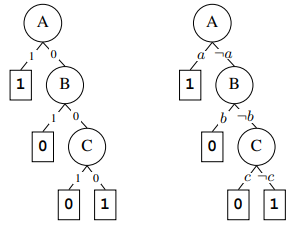
\includegraphics[width=0.9\linewidth]{graph}
	\caption{Optimal tree corresponding to database of Table 1. Max depth = 3 and minimum examples per leaf = 1}
	\label{fig:1}
\end{figure}
Using this representation, every path in a decision tree can be mapped to an itemset $I \subseteq \mathcal{I}$, as shown in Figure \ref{fig:1b}. For instance, the last path in this tree corresponds to the itemset $\{\neg a, \neg b, \neg c\}$. Please note that multiple paths can be mapped
to the same itemset.

For every itemset $I$, we define its cover to be $cover (I) = \{(t', I' , c') \in \mathcal{D} | I \subseteq I'\}$ : the set of transactions in which the itemset is contained; the class-based support of an itemset is defined as $Sup(I, c) = |\{(t', I', c')\in cover (I)| c' = c\}|$, and can be used to identify the number of examples for a given class c in a leaf. Based on class-based supports, the error of an itemset is defined as:
\begin{equation}
	leaf\_error(I) =| cover(I) | - \max_{c\in\mathcal{C}}\{Sup(I,c)\}
	\label{eq:1}
\end{equation}

Unlike the CP-based approach, our error function is also valid for classification tasks involving more than 2 classes.

The canonical decision tree learning problem that we
study in this work can now be defined as follows using itemset mining notation. Given a database $\mathcal{D}$, we wish to identify a collection $\mathcal{DT} \subseteq \mathcal{I}$ of itemsets such that
\begin{itemize}
	\item the itemsets in DT represent a decision tree;
	\item $\sum_{I\in\mathcal{DT}} leaf\_error(I)$ is minimal;
	\item for all $I\in\mathcal{DT} : |I| \le maxdepth$, where $maxdepth$ is the maximum depth of the tree;
	\item for all $I\in\mathcal{DT} :| cover(I) \ge minsup$, where $minsup$ is a minimum support threshold.
\end{itemize}
As stated earlier, in DL8, the maximum depth constraint is not required; MIP-based approaches have ignored the minimum support constraint.

	\section{DL8 Algorithm}
%\newcommand{\Proc}[1]{\textbf{Procedure #1}}
\begin{algorithm}
	\DontPrintSemicolon
	\caption{$DL8(maxdepth, minsup)$}
	\label{algo:1}
	\textbf{struct} $BestTree\{\ tree : Tree; error : float\ \}$\;
	$cache \gets HashSet < Itemset, BestTree >$\;
	$(\tau, b) \gets \verb|DL8-Recurse|(\emptyset)$\;
	\Return $\tau$\;
	\textbf{Procedure} \texttt{DL8-Recurse}$(I)$\;
		$solution \gets cache.get(I)$\;
		\If{solution was found}{
			\Return($solution.tree, solution.error$)\;
		}
		\If{$leaf\_error(I) = 0\ or\ |I| = maxdepth$}{
			\Return($make\_leaf(I), leaf\_error (I)$)\;
		}
		$(\tau, b) \gets (make\_leaf(I), leaf\_error (I))$\;
		\For{all attributes $i$}{
			\If{$|cover (I \cup \{i\})| \ge minsup$ and $|cover (I \cup \{\neg i\})| \ge minsup$}{
				$(\tau_1, e_1) \gets \texttt{DL8-Recurse}(I \cup \{i\})$\;
				\If{$e_1 \le b$}{
					$(\tau_2, e_2) \gets \texttt{DL8-Recurse}(I \cup \{i\})$\;
					\If{$e_1 + e_2 \le b$}{
						$(\tau, b) \gets (make\_tree(i, \tau_1, \tau_2), e_1 + e_2)$\;
					}
				}
			}
		}
		$cache.store(I, BestT ree(\tau, b))$\;
		\Return($\tau, b$)\;
\end{algorithm}

A high-level perspective of the DL8 algorithm is given in Algorithm \ref{algo:1}. Essentially, the algorithm recursively enumerates itemsets using the \verb|DL8-Recurse(I)| function. The post-condition of this function is that it returns the optimal decision tree for the transactions covered by itemset $I$, together with the quality of that tree. This optimal tree is calculated recursively using the observation that the best decision tree for a set of transactions can be obtained by considering all possible ways of partitioning the set of transactions into two, and determining the best tree for each partition recursively.

Figure \ref{fig:2} illustrates the search space of itemsets for the dataset of Table \ref{tab:1}, where all the possible itemsets are represented. Intuitively, DL8 starts at the top node of this search space, and calculates the optimal decision tree for the root based on its children.

A distinguishing feature of DL8 is its use of a cache. The idea behind this cache is to store the result of a call to \verb|DL8-Recurse(I)|. Doing so is effective as the same itemset can be reached by multiple paths in the search space: itemset $ab$ can be constructed by adding $b$ to itemset $a$, or by adding $a$ to itemset $b$. By storing the result, we can reuse the same result for both paths.

Note that the optimal decision tree for the root can only be calculated after all its children have been considered; hence, the algorithm will only produce a solution once the entire search space of itemsets has been considered.

In our pseudocode, we use the following other functions. Function $make\_leaf(I)$ returns a decision tree with one node, representing a leaf that predicts the majority class for the examples covered by I. The function $make\_tree(i, \tau_1, \tau_2)$ returns a tree with a test on attribute $i$, and subtrees $\tau_1$ and $\tau_1$.

The code illustrates a number of optimizations implemented in DL8:
\begin{description}
	\item[Maximum depth pruning] In line 9 the search is stopped as soon as the itemsets considered are too long;
	\item[Minimum support pruning] In line 13 an attribute is not considered if one of its branches has insufficient support ; in our running example, the itemset $\{a, b, c\}$ is not considered due to this optimization;
	\item[Purity pruning] In line 9 the search is stopped if the error for the current itemset is already 0;
	\item[Quality bounds] In the loop of lines 12–18, the best solution found among the children is maintained, and used to prune the second branch for an attribute if the first branch is already worse than the best solution found so far.
\end{description}
 
We omit a number of optimizations in this pseudo-code that can be found in the original publication, in particular, optimizations that concern the incremental maintenance of data structures. While we will use most of these optimizations in our implementation as well, we do not discuss thesein detail here for reasons of simplicity.

The most important optimization in DL8 that we do not use in this study is the \emph{closed itemset mining} optimization. The reason for this choice is that this optimization is hard to combine with a constraint on the depth of a decision tree. Similarly, while DL8 can be applied to other scoring functions than error, as long as the scoring function is \emph{additive}, we prioritize accuracy and the depth constraint here as we focus on solving the same problem as in recent MIP-based studies.
\begin{figure*}
	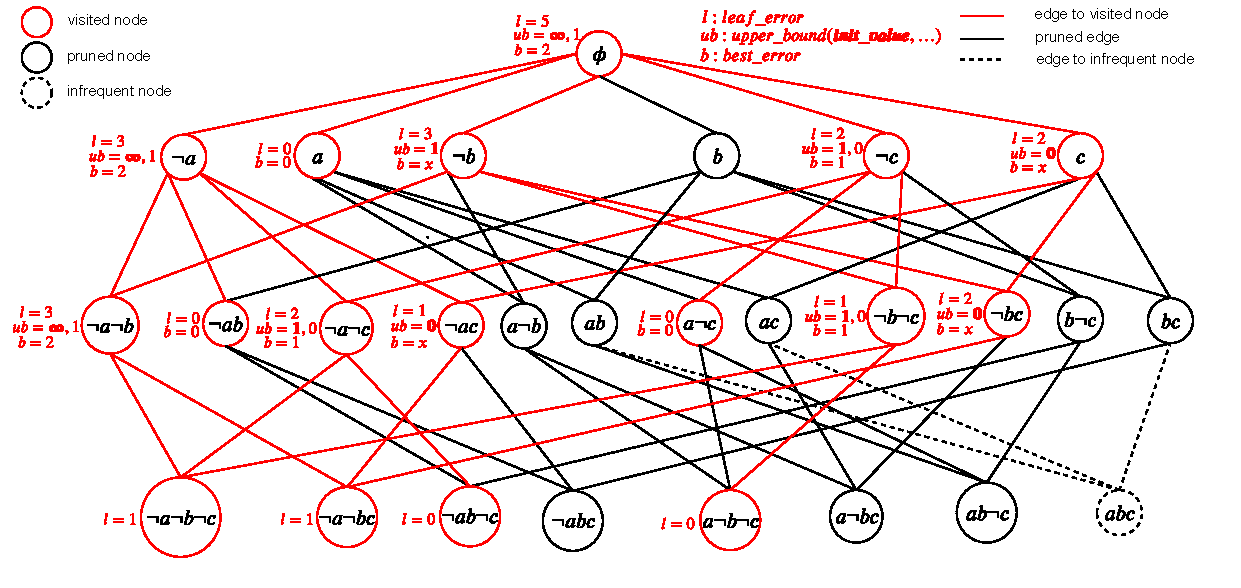
\includegraphics[width=\textwidth]{images/lattice_search}
	\caption{: Complete itemset lattice for introduction database and DL8.5 search execution}
	\label{fig:2}
\end{figure*}


	\section{Our approach: DL8.5}
As identified in the introduction, DL8 has a number of weaknesses, which we will address in this section.

The most prominent of these weaknesses is that the size of the search tree considered by DL8 is unnecessarily large. Reconsider the example of Figure \ref{fig:2}, in which DL8’s pruning approach does not prune any node except from one infrequent itemset $(abc)$. We will see in this section that a new type of caching brand-and-bound search can reduce the number of itemsets considered significantly.

The pseudo-code of our new algorithm, DL8.5, is presented in Algorithm \ref{algo:2}. DL8.5 inherits a number of ideas from DL8, including the use of a cache, the recursive traversal of the space of itemsets, and the use of depth and support constraints to prune the search space.

The main distinguishing feature of DL8.5 concerns its use of bounds during the search.

In DL8.5, the recursive procedure \verb|DL8.5-Recurse| has an additional parameter, \emph{init\_ub}, which represents an upper-bound on the quality of the decision trees that the recursive procedure is expected to find. If no sufficiently good tree can be found, the procedure returns a tree of type \verb|NO TREE|. Initially, the upper-bound that is used is $+\infty$ (line 3). However, as soon as the recursive algorithm has found one decision tree, or has found a better tree than earlier known, the quality of this decision tree, calculated in line 21, is used as upper-bound for future decision trees and is communicated to the children in the search tree (line 25, line 14, 18).

The upper-bound is used to prune the search space using a test in line 17; intuitively, as soon as we have traversed one branch for an attribute, and the quality of that branch is already worse than accepted by the bound, we do not consider the second branch for that attribute.

\newcommand{\trmtt}[1]{\textrm{\texttt{#1}}}
\begin{algorithm}
	\DontPrintSemicolon
	\caption{$DL8.5(maxdepth, minsup)$}
	\label{algo:2}
	\label{algo:1}
	\textbf{struct} $BestTree\{init\_ub : float;\ tree: Tree;\ error : float\}$\;
	$cache \gets HashSet < Itemset, BestTree >$\;
	$bestSolution \gets$ \verb|DL8-Recurse|$(\emptyset, \infty)$\;
	\Return bestSolution.tree\;
	\textbf{Procedure} \texttt{DL8-Recurse}$(I, init\_ub)$\;
	\Procb{
		\If{$leaf\_error(I) = 0$ or $|I| = maxdepth$ or time-out
			is reached}{
			\Return $BestTree(init\_ub, make\_leaf (I),$ $leaf\_error (I))$\;
		}
		$solution \gets cache.get(I)$\;
		\If{solution was found and (($solution.tree \ne$ \textrm{\texttt{NO\_TREE}}) or $(init\_ub \le solution.init\_ub)$) }{
			\Return $solution$\;
		}
		$(\tau, b, ub) \gets (\mathrm{\mathtt{NO\_TREE}}, +\infty, init\_ub)$\;
		\For{all attributes $i$ in a well-chosen order}{
			\If{$|cover (I \cup \{i\})| \ge minsup$ and $|cover (I \cup \{\neg i\})| \ge minsup$}{
				$sol_1 \gets \textrm{\texttt{DL8.5-Recurse}}(I \cup \{i\}, ub)$\;
				\If{$sol_1.tree =\mathrm{\mathtt{NO\_TREE}}$}{
					\textbf{continue}\;
				}
				\If{$sol_1.error \le ub$}{
					$sol_2 \gets \mathtt{DL8.5-Recurse}(I \cup \{i\},$ ${ub-sol_1.error})$\;
					\If{$sol_2.tree =\mathrm{\mathtt{NO\_TREE}}$}{
						\textbf{continue}\;
					}
					$feature\_error \gets sol_1.error + sol_2.error$\;
					\If{$feature\_error \le ub$}{
						$\tau \gets make\_tree(i, sol_1.tree,$ $sol_2.tree)$\;
						$b \gets feature\_error$\;
						$ub \gets b - 1$\;
					}
					\If{$feature\_error = 0$}{\textbf{break}}
				}
			}
		}
		$solution \gets BestTree(init\_ub, \tau, b)$\;
		$cache.store(I, solution)$\;
		\Return $solution$\;
	}
\end{algorithm}
In line 18 we use the quality of the first branch to bound the required quality of the second branch further.

An important modification involves the interaction of the bounds with the cache. In DL8.5, we store an itemset also if no solution could be found for the given bound (line 29 is still executed even if the earlier loop did not find a tree).

In this case, the special value \verb|NO_TREE| is associated with the itemset in the cache, and the upper-bound used during the last search is stored. The benefit of doing so is that at a later moment, we may reuse the fact that for a given itemset and bound, no sufficiently good decision tree can be found. In particular, in line 9, when the current bound (\emph{init\_ub}) is worse than the stored upper-bound for a \verb|NO TREE| itemset, we return the \verb|NO TREE| indicator immediately.

Other modifications in comparison with DL8 improve the anytime behavior of the algorithm. In line 6 the search can be interrupted when a time-out is reached, and line 12 offers the possibility to consider the attributes in a specific heuristic order to discover good trees more rapidly.

A number of different heuristics could be considered. In our experiments, we consider three: the original order of the attributes in the data, in increasing or in decreasing order of information gain (such as used in C4.5 and CART).

Our modifications of DL8 improve drastically the pruning of the search space. Figure \ref{fig:2} indicates which additional nodes are pruned during the execution of DL8.5 (for an alphabetic order of the attributes). At the end, 17 nodes are visited instead of 27.

\begin{figure}
	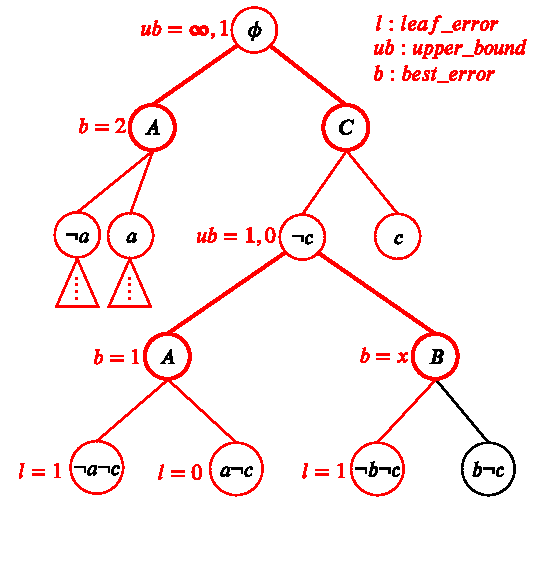
\includegraphics[width=\linewidth]{pruning}
	\caption{ Example of pruning}
	\label{fig:3}
\end{figure}

Figure \ref{fig:3} shows a part of the execution of DL8.5 in more detail. The initial value of the upper-bound at node $\phi$ is $+\infty$ (line 11). The attribute A provides an error of 2; the upper-bound value is subsequently updated from $+\infty$ to 1 in line 25. In the first branch for attribute C, the new value of the upper-bound is passed down recursively (line 14). Notice that the initial value of the upper-bound at node $\neg c$ is 1. At this node, the attribute A is first visited and provides an error of 1 by summing errors of $\neg a\neg c$ and $a\neg c$ (line 21). The upper-bound for subsequent attributes is then updated to 0 and passed down recursively to the first branch of attribute B. After visiting the first item $\neg b\neg c$ the obtained error is 1 and greater than the upper-bound of 0. The second item is pruned as the condition of line 18 is not satisfied. So, there is no solution by selecting the attribute B, which leads to storing the value \verb|NO TREE| for this itemset. This error value is represented in Figures 2 and 3 by the character x.

The reuse of the cache is illustrated for itemset $\neg ac$ (Figure \ref{fig:2}). The first time we encounter this itemset, we do so coming from the itemset $\neg a$ for an upper-bound of zero; after the first branch, we observe that no solution can be found for this bound, and we store \verb|NO TREE| for this itemset. The second time we encounter $\neg ac$, we do so coming from the parent c, again with an upper-bound of 0. From the cache we retrieve the fact that no solution could be found for this bound, and we skip attribute A from further consideration.
	\section{Results}
In our experiments we answer the following questions:
\begin{description}
	\item[Q1] How does the performance of DL8.5 compare to DL8, MIP-based and CP-based approaches on binary data?
	\item[Q2] What is the impac\emph{TO}f different branching heuristics on the performance of DL8.5?
	\item[Q3] What is the impac\emph{TO}f caching incomplete results in DL8.5 (NO TREE itemsets)?
	\item[Q4] How does the performance of DL8.5 compare to DL8, MIP-based and CP-based approaches on continuous data?
\end{description}
As a representative MIP-based approach, we use BinOCT, as it was shown to be the best performing MIP-based approach in a recent study (Verwer and Zhang 2019). The implementations of BinOCT\footnote{https://github.com/SiccoVerwer/binoct}, DL8 and the CP-based approach\footnote{https://bitbucket.org/helene\_verhaeghe/classificationtree/src/ default/classificationtree/} used in our comparison were obtained from their original authors, and use the CPLEX 12.9\footnote{https://www.ibm.com/analytics/cplex-optimizer} and OscaR\footnote{https://oscarlib.bitbucket.io} solvers. Experiments were performed on a server with an Intel Xeon E5-2640 CPU, 128GB of memory, running Red Hat 4.8.5-16.

To respect the constrain\emph{TO}f the CP-based algorithm all the datasets used in our experiments have binary classes. We compare our algorithms on 24 binary datasets from CP4IM\footnote{https://dtai.cs.kuleuven.be/CP4IM/datasets/}, described in the first columns of Table \ref{tab:2}.

Similar to Verwer and Zhang (2019), we run the different algorithms for 10 minutes on each dataset and for a maximum depth of 2, 3 and 4. All the tests are run with a minimum suppor\emph{TO}f 1 since this is the setting used in BinOCT.

We do not spli\emph{TO}ur datasets in training and test sets since the focus of this work is on comparing the computational performance of algorithms that should generate decision trees of the same quality. The benefits of optimal decision trees were discussed in (Bertsimas and Dunn 2017).

We compare a number of variants of DL8.5. The following table summarizes the abbreviations used.

\noindent\begin{tabularx}{\linewidth}{lX}
	Abbreviation	& Meaning		\\\hline
	d.o.			& the original order of the attributes in the data is used as branching heuristic		\\
	asc				& attributes are sorted in increasing value of information gain		\\
	desc			& attributes are sorted in decreasing value of information gain		\\
	n.p.s.			& no partial solutions are stored in the cache
\end{tabularx}

Table \ref{tab:2} shows the results for a maximum depth equal to 4, as we consider deeper decision trees of more interest. If optimality could not be proven within 10 minutes, this is indicated using \emph{TO}; in this case, the objective value of the best tree found so far is shown. Note that we here exploit the ability of DL8.5 to produce a result after a time-out. The best solutions and best times are marked in bold while a star (*) is added to mark solutions proven to be optimal.

BinOCT solved and proved optimality for only 1 instance within the timeout; the older DL8 algorithm solved 7 instances and the CP-based algorithm solved 11 instances. DL8.5 solved 19 (which answers \textbf{Q1}). The difference in performance is further illustrated in Figure \ref{fig:4}, which gives \emph{cactus plots} for each algorithm, for different depth constraints. In these plots each point $(x, y)$ indicates the number of instances $(x)$ solved within a time limit $(y)$. While for lower depth thresholds, BinOCT does find solutions, the performance of all variants of DL8.5 clearly remains superior to tha\emph{TO}f DL8, BinOCT and the CP-based algorithm, obtaining orders of magnitude better performance.

Comparing the different branching heuristics in DL8.5, the differences are relatively small; however, for deeper trees, a descending order of information gain gives slightly better results. This confirms the intuition that chosen a split with high information gain is a good heuristic (\textbf{Q2}).

If we disable DL8.5’s ability to cache incomplete results, we see a significant degradation in performance. In this varian\emph{TO}nly 12 instances are solved optimally, instead of 19, for a depth of 4. Hence, this optimization is significant (\textbf{Q3}).

To answer \textbf{Q4}, we repeat these tests on continuous data. For this, we use the same datasets as Verwer and Zhang (2019). These datasets were obtained from the UCI repository\footnote{https://archive.ics.uci.edu/ml/index.php} and are summarized in the first columns of Table \ref{tab:3}. Before running DL8, the CP-based algorithm and DL8.5, we binarize these datasets by creating binary features using the same approach as the one used by \cite{verwer:2019learning}. %Verwer and Zhang (2019).
Note that the number of generated features is very high in this case. As a result, for most datasets all algorithms reach a time-out for maximum depths of 3 and 4, as was also shown by Verwer and Zhang (2019). Hence, we focus on results for a depth of 2 in Table \ref{tab:3}. Even though BinOCT uses a specialized technique for solving continuous data, the table shows that DL8.5 outperforms DL8, the CP-based algorithm and BinOCT. Note that the differences between the different variations of DL8.5 are small here, which may not be surprising given the shallowness of the search tree considered.

\begin{table*}
	\tiny\centering
	\begin{tabular}{|L{0.08\linewidth}|*{10}{C{0.03\linewidth}|}|*{2}{C{0.03\linewidth}|}|*{2}{C{0.03\linewidth}|}|*{2}{C{0.03\linewidth}|}}
		\hline
		\multirow{3}{*}{Dataset}	& \multirow{3}{*}{nItems}	 & \multirow{3}{*}{nTrans}	& \multicolumn{2}{c|}{BinOCT} &\multicolumn{2}{c|}{DL8}	&\multicolumn{2}{c|}{CP-Based}	& \multicolumn{8}{c|}{DL8.5}		\\
		& 	 & 	& & &&	&&	& \multicolumn{2}{c||}{d.o.}	& \multicolumn{2}{c||}{asc}	& \multicolumn{2}{c||}{desc}	& \multicolumn{2}{c|}{n.p.s.}		\\
		& 	 & 	& \rotatebox{90}{obj} & \rotatebox{90}{time (s)} & \rotatebox{90}{obj}& \rotatebox{90}{time (s)}	& \rotatebox{90}{obj}	& \rotatebox{90}{time (s)}	& \rotatebox{90}{obj}	& \rotatebox{90}{time (s)}	& \rotatebox{90}{obj}	& \rotatebox{90}{time (s)}	& \rotatebox{90}{obj}	& \rotatebox{90}{time (s)}	&\rotatebox{90}{obj}	& \rotatebox{90}{time (s)}	\\
		\hline\hline
		anneal	& 186 	& 812	& 115	& $TO$	& $\infty$	& $TO$	&\bf 91*	&\bf 450.69	&\bf 91*	& 129.24	&\bf 91*	& 127.45	&\bf 91*	& 121.87	& 91*	& 250.64		\\
		\hline
		audiology	& 296	& 216	& 2	& \emph{TO}	& $\infty$	& \emph{TO}	& 1	& \emph{TO}	& 1*	& 180.84	& 1*	& 204.19	& 1*	& 195.73	& 1	& \emph{TO}		\\
		\hline
		australian-credit	& 250	& 653	& 82	& \emph{TO}	& $\infty$	& \emph{TO}	& 66	& \emph{TO}	&\bf 56*	& 566.71	&\bf 56*	& 586.39	&\bf 56*	& 593.38	& 57	& \emph{TO}		\\
		\hline
		breast-wisconsin	& 240	& 683	& 12	& \emph{TO}	& $\infty$	& \emph{TO}	& 8	& \emph{TO}	&\bf 7*	& 305.3	&\bf 7*	& 325.7	&\bf 7*	& 330.71	& 7	& \emph{TO}		\\
		\hline
		diabetes	& 224	& 768	& 170	& \emph{TO}	& $\infty$	& \emph{TO}	& 140	& \emph{TO}	&\bf 137*	& 553.49	&\bf 137*	& 562.83	&\bf 137*	& 565.5	& 137	& \emph{TO}			\\
		\hline
		german-credit	& 224	& 1000	& 223	& \emph{TO}	& $\infty$	& \emph{TO}	& 204	& \emph{TO}	&\bf 204*	& 558.73	& 206	& \emph{TO}	&\bf 204*	& 599.87	& 204	& \emph{TO}		\\
		\hline
		heart-cleveland	& 190	& 296	& 39	& \emph{TO}	& $\infty$	& \emph{TO}	& 25	& \emph{TO}	&\bf 25*	& 124.1	&\bf 25*	& 130.3	&\bf 25*	& 132.23	&\bf 25*	& 214.76	    \\
		\hline
		hepatitis	& 136	& 137	& 7	& \emph{TO}	&\bf 3*	& 66.62	&\bf 3*	& 109.36	& \bf 3*	& 13.46	& \bf 3*	& 14.06	& \bf 3*	& 14.88	& \bf 3*	& 27.28         \\
		\hline
		hypothyroid	& 176	& 3247	& 55	& \emph{TO}	& $\infty$	& \emph{TO}	& 53	& \emph{TO}	&\bf 53*	& 392.22	&\bf 53*	& 368.95	&\bf 53*	& 427.34	& 53	& \emph{TO}	    \\
		\hline
		ionosphere	& 890	& 351	& 27	& \emph{TO}	& $\infty$	& \emph{TO}	& 20	& \emph{TO}	& 17	& \emph{TO}	& 11	& \emph{TO}	& 13	& \emph{TO}	& 17	& \emph{TO}       \\
		\hline
		kr-vs-kp	& 146	& 3196	& 193	& \emph{TO}	& $\infty$	& \emph{TO}	&\bf 144*	& 483.15	&\bf 144*	& 216.11	&\bf 144*	& 206.18	&\bf 144*	& 223.85	&\bf 144*	& 528.72        \\
		\hline
		letter	& 448	& 20000	& 813	& \emph{TO}	& $\infty$	& \emph{TO}	& 574	& \emph{TO}	& 550	& \emph{TO}	& 586	& \emph{TO}	& 802	& \emph{TO}	& 550	& \emph{TO}       \\
		\hline
		lymph	& 136	& 148	& 6	& \emph{TO}	&\bf 3*	& 56.29	&\bf 3*	& 112.48	&\bf 3*	& 8.7	&\bf 3*	& 11.03	&\bf 3*	& 8.47	&\bf 3*	& 25.04     \\\hline
		mushroom	& 238	& 8124	& 278	& \emph{TO}	& $\infty$	& \emph{TO}	&\bf 0*	& 352.18	&\bf 0*	& 331.39	& 4	& \emph{TO}	&\bf 0*	& 0.11	& 4	& \emph{TO}	    \\
		\hline
		pendigits	& 432	& 7494	& 780	& \emph{TO}	& $\infty$	& \emph{TO}	& 38	& \emph{TO}	& 32	& \emph{TO}	& 26	& \emph{TO}	& 14	& \emph{TO}	& 32	& \emph{TO}       \\
		\hline
		primary-tumor	& 62	& 336	& 37	& \emph{TO}	&\bf 34*	& 2.79	&\bf 34*	& 8.96	&\bf 34*	& 1.48	& \bf34*	& 1.51	& 34*	& 1.38	&\bf 34*	& 2.43      \\
		\hline
		segment	& 470	& 2310	& 13	& \emph{TO}	& $\infty$	& \emph{TO}	&\bf 0*	& 128.25	&\bf 0*	& 3.54	&\bf 0*	& 6.99	&\bf 0*	& 7.05	&\bf 0*	& 3.54      \\
		\hline
		soybean	& 100	& 630	& 15	& \emph{TO}	&\bf 14*	& 41.59	&\bf 14*	& 40.13	&\bf 14*	& 5.7	&\bf 14*	& 6.34	&\bf 14*	& 5.75	&\bf 14*	& 18.41     \\
		\hline
		splice-1	& 574	& 319	& 574	& \emph{TO}	& $\infty$	& \emph{TO}	& $\infty$	& \emph{TO}	& 224	& \emph{TO}	& 224	& \emph{TO}	& 141	& \emph{TO}	& 224	& \emph{TO}       \\
		\hline
		tic-tac-toe	& 54	& 958	& 180	& \emph{TO}	&\bf 137*	& 3.76	&\bf 137*	& 9.17	&\bf 137*	& 1.43	&\bf 137*	& 1.54	&\bf 137*	& 1.55	&\bf 137*	& 2.12      \\
		\hline
		vehicle	& 504	& 846	& 61	& \emph{TO}	& $\infty$	& \emph{TO}	& 22	& \emph{TO}	& 16	& \emph{TO}	& 18	& \emph{TO}	& 13	& \emph{TO}	& 16	& \emph{TO}       \\
		\hline
		vote	& 96	& 435	& 6	& \emph{TO}	&\bf 5*	& 29.84	&\bf 5*	& 44.47	&\bf 5*	& 5.48	&\bf 5*	& 5.33	&\bf 5*	& 5.58	&\bf 5*	& 12.82     \\
		\hline
		yeast	& 178	& 1484	& 395	& \emph{TO}	& $\infty$	& \emph{TO}	& 366	& \emph{TO}	&\bf 366*	& 318.87	&\bf 366*	& 326.2	&\bf 366*	& 334.15	&\bf 366*	& 470.88        \\
		\hline
		zoo-1	& 72	& 101	&\bf 0*	& 0.52	&\bf 0*	& 1.11	&\bf 0*	& 0.2	&\bf 0*	& 0.01	&\bf 0*	& 0.01	&\bf 0*	& 0.01	&\bf 0*	& 0.01      \\
		\hline
	\end{tabular}
	\caption{: Comparison table for binary datasets with max depth = 4}
	\label{tab:2}
\end{table*}
\begin{figure*}
	\centering
	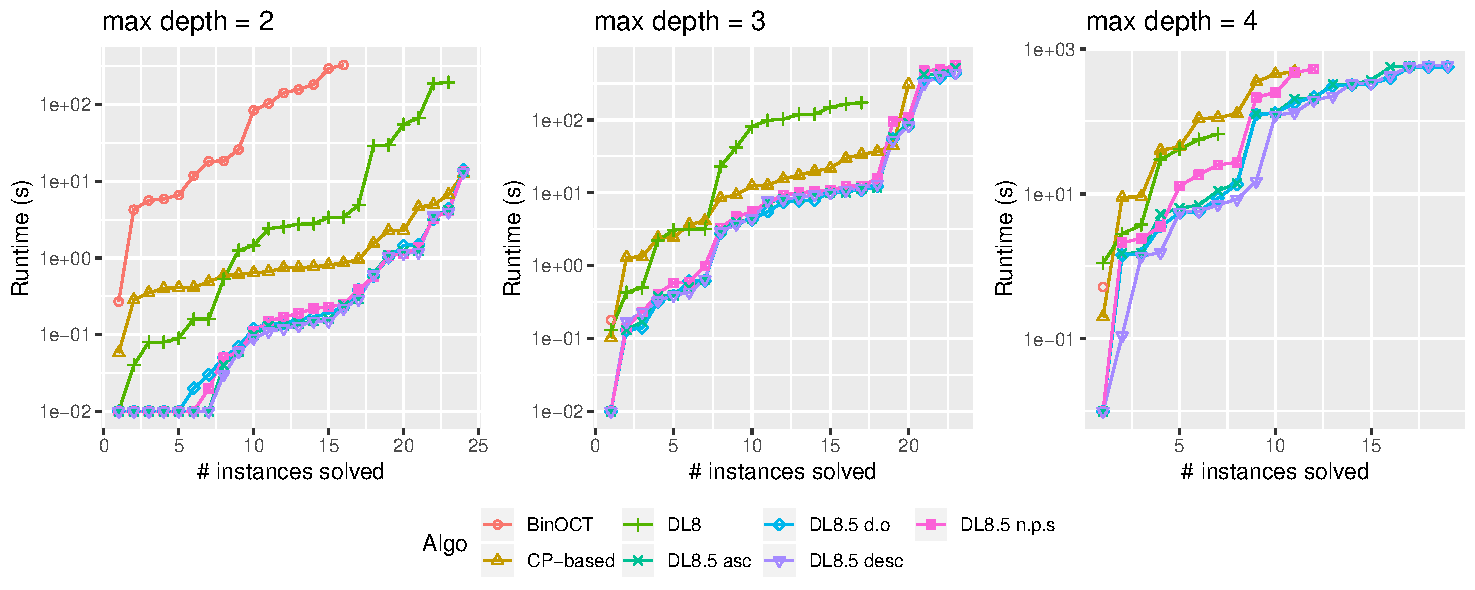
\includegraphics[width=0.9\linewidth]{cactus_log}
	\caption{Cumulative number of instances solved over time}
	\label{fig:4}
\end{figure*}
\begin{table*}
	\tiny\centering
	\begin{tabular}{|L{0.08\linewidth}|*{11}{C{0.03\linewidth}|}|*{2}{C{0.03\linewidth}|}|*{2}{C{0.03\linewidth}|}}
		\hline
		\multirow{3}{*}{Dataset}	& \multirow{3}{*}{nTrans}	 & \multirow{3}{*}{nFeat}	& \multirow{3}{*}{nItems}	& \multicolumn{2}{c|}{BinOCT} &\multicolumn{2}{c|}{DL8}	&\multicolumn{2}{c|}{CP-Based}	& \multicolumn{6}{c|}{DL8.5}		\\
		& 	 & 	& & &&	&&	&& \multicolumn{2}{c||}{d.o.}	& \multicolumn{2}{c||}{asc}	& \multicolumn{2}{c||}{desc}		\\
			& 	 & 	&& \rotatebox{90}{obj} & \rotatebox{90}{time (s)} & \rotatebox{90}{obj}& \rotatebox{90}{time (s)}	& \rotatebox{90}{obj}	& \rotatebox{90}{time (s)}	& \rotatebox{90}{obj}	& \rotatebox{90}{time (s)}	& \rotatebox{90}{obj}	& \rotatebox{90}{time (s)}	& \rotatebox{90}{obj}	& \rotatebox{90}{time (s)}		\\
		\hline\hline
		balance-scale   & 625   & 4 & 32  & \bf 149* & 1.2 & \bf 149*    & 0.5    & \bf 149*   & 0.01  & \bf 149* & 0.01    & \bf 149*   & 0.01  & \bf 149* & 0.01\\
		\hline
		banknote  & 1372  & 4	& 3710  & 101  & \emph{TO}  & \bf 100*  & 363.01  & $\infty$  & \emph{TO}  & \bf 100*  & 52.81  & \bf 100*  & 63.41  & \bf 100*  & 58.07\\
		\hline
		bank  & 4521  & 51  & 3380  & 449  & \emph{TO}  & 448  & \emph{TO}  & $\infty$  & \emph{TO}  & \bf 44\bf 6*  & 253.87  & \bf 44\bf 6*  & 223.42  & \bf 44\bf 6*  & 222.66\\
		\hline
		biodeg  & 1055  & 41  & 8356  & 212  & \emph{TO}  & 212  & \emph{TO}  & $\infty$  & \emph{TO}  & \bf 202*  & 341.57  & \bf 202*  & 365.83  & \bf 202*  & 370.26\\
		\hline
		car  & 1728  & 6  & 28   & \bf 250*  & 4.09  & \bf 250*  & 0.32  & \bf 250*  & 0.02  & \bf 250*  & 0.01  & \bf 250*  & 0.01  & \bf 250*  & 0.01\\
		\hline
		IndiansDiabetes  & 768  & 8  & 1714  & 171  & \emph{TO}  & \bf 171*  & 36.75  & $\infty$  & \emph{TO}  & \bf 171*  & 7.43  & \bf 171*  & 8.46  & \bf 171*  & 8.72\\
		\hline
		Ionosphere  & 351  & 34  & 4624  & 29  & \emph{TO}  & \bf 29*  & 423.52  & $\infty$   & \emph{TO}  & \bf 29*  & 25.68  & \bf 29*  & 33.76  & \bf 29*  & 33.04\\
		\hline
		iris  & 150  & 4  & 52  & \bf 0*  & 0.02  & \bf 0*  & 0.05  & \bf 0*  & 0.01  & \bf 0*  & 0.01  & \bf 0*  & 0.01  & \bf 0*  & 0.01\\
		\hline
		letter    & 20000    & 16    & 352    & 625    & \emph{TO}    & \bf 591*    & 5.97    & \bf 591*    & 392.09    & \bf  591*    & 8.61    & \bf 591*    & 8.26    & \bf 591*    & 8.83\\
		\hline
		messidor    & 1151    & 19    & 9460    & 383    & \emph{TO}    & 383    & \emph{TO}    & $\infty$    & \emph{TO}    & 383*    & 533.27    & 383*    & 563.83    & 383*    & 534.32\\
		\hline
		monk1    & 124    & 6    & 22    & 22*    & 0.33    & 22*    & 0.28    & 22*    & 0.01    & 22*    & 0.01    & 22*    & 0.01    & 22*    & 0.01\\
		\hline
		monk2    & 169    & 6    & 22    & 57*    & 0.79    & 57*    & 0.28    & 57*    & 0.01    & 57*    & 0.01    & 57*    & 0.01    & 57*    & 0.01\\
		\hline
		monk3    & 122    & 6    & 22    & 8*    & 0.31    & 8*    & 0.28    & 8*    & 0.01    & 8*    & 0.01    & 8*    & 0.01    & 8*    & 0.01\\
		\hline
		seismic    & 2584    & 18    & 2240    & 166    & \emph{TO}    & 164*    & 117.34    & $\infty$    & \emph{TO}    & 164*    & 44.3    & 164*    & 47.36    & 164*    & 47.17\\
		\hline
		spambase    & 4601    & 57    & 16012    & 660    & \emph{TO}    & 900    & \emph{TO}    & $\infty$    & \emph{TO}    & 741    & \emph{TO}    & 845    & \emph{TO}    & 586    & \emph{TO}\\
		\hline
		Statlog    & 4435    & 36    & 3274    & 460    & \emph{TO}    & 443    & \emph{TO}    & $\infty$    & \emph{TO}    & 443*    & 205.14    & 443*    & 193.87    & 443*    & 188.9\\
		\hline
		tic-tac-toe    & 958    & 18    & 36    & 282*    & 7.52    & 282*    & 0.33    & 282*    & 0.01    & 282*    & 0.01    & 282*    & 0.01    & 282*    & 0.01\\
		\hline
		wine    & 178    & 13    & 1198    & 6*    & 73.1    & 6*    & 7.0    & 6*    & 74.72    & 6*    & 1.17    & 6*    & 1.45    & 6*    & 1.09\\
		\hline
	\end{tabular}
	\caption{ Comparison table for continuous datasets with max depth = 2}
	\label{tab:3}
\end{table*}
	\section{Conclusions}
In this paper we presented the DL8.5 algorithm for learning optimal decision trees. DL8.5 is based on a number of ideas: the use of itemsets to represent paths, the use of a cache to store intermediate results (including results for parts ofthe search tree that have only been traversed partially), theuse of bounds to prune the search space, the ability to useheuristics during the search, and the ability to return a resulteven when a time-out is reached.

Our experiments demonstrated that DL8.5 outperforms existing approaches by orders of magnitude, including approaches presented recently at prominent venues.
In this paper, we focused our experiments on one particular setting: learning maximally accurate trees of limited depth without support constraints. This was motivated by our desire to compare our new approach with other approaches. However, we believe DL8.5 can be modified for use in other constraint-based decision tree learning problems, using ideas from DL8 (Nijssen and Fromont 2010).\\
\textbf{Acknowledgements}. This work was supported by Bpost.
	
	\bibliography{Bibliography-File}
	\bibliographystyle{settings/aaai}
\end{document}